\chapter{Cadre général du projet}
\section{Introduction}
Dans ce chapitre, nous allons présenter le cadre du projet. En premier lieu, nous proposerons une présentation de l'entreprise d'accueil Linedata. Ensuite nous présenterons une critique de la solution existante ainsi que les solutions proposées. Et nous clôturons ce chapitre par une exposition de la méthodologie suivie tout au long de la réalisation du projet.
\section{Présentation de l'organisme d'accueil}
Linedata est un éditeur de solutions globales qui travaille dans le secteur de management, de l'assurance et du crédit. Chaque jour, plus de 63000 professionnels financiers opérant dans 50 pays font confiance à ses technologies afin de gérer leurs activités. Le logo de l'organisme d'accueil est présenté par la Figure \ref{code1}
\begin{figure}[h]
  \centering
  
\includegraphics[scale=0.3]{figures/linedatalogo.png}
  \caption{Logo Linedata}
  \label{code1}
\end{figure}

\subsection{Historique}
Linedata est né en janvier 1998 du rapprochement de trois sociétés: \textbf{Générale de service informatique (GSI) Division des Banques}, \textbf{Line Data} et \textbf{BDB Participation}.\\

GSI Division des banques a été rachetée majoritairement par ses salariés au mois de décembre 1997. L'accquisition ultérieure de Line Data et de BDB Participation a permis la constition d'une nouvelle société: \textbf{Linedata Services}.

Cette dernière n'est pas donc une création de toutes pièces mais elle avait dès ses débuts du savoir-faire humain et technologique ce qui lui a permis en 17 mai 2000 d'être introduit en bourse sur le Nouveau Marché de la Bourse de Paris. Linedata est ainsi depuis 10 ans une société cotée sur Euronext Paris.\\

Linedata s'est rapidement développé pour accompagner ses clients en élargissant son offre produit tout en ciblant de nouveaux marchés. Afin d'accompagner sa croissance, Linedata a mis en place une stratégie d'acquisition et d'intégration réussie depuis plus de 15 ans:\\
\begin{itemize}
    \item[$\bullet$] Février 2000: Les sociétés Bimaco Finance, Pen Lan et EKIP/Ingénétudes qui sont basées à Paris ont permis à Linedata d'appuyer sa leadership dans le domaine des crédits et financement.\\
    \item[$\bullet$] Février 2003: Acquisition des solutions Icon et Préview qui permettent la gestion de protefeuilles. Ils ont permis au groupe de rejoindre la tête du classement au Royaume-Uni et de consolider sa position de numéro 1 en Europe.\\
    \item[$\bullet$] Décembre 2003: Acquisition de Economic and Social Data Service Solutions (ESDS) qui est un des spécialistes français dans le domaine des progiciels d'assurance individuelle. Ceci a permis à Linedata Services d'être en 2004 un acteur majeur dans le domaine d'Epargne Retraite et la Prévoyance tout en se positionnant significativement sur le segment en très forte croissance des assurances de personnes.\\
    \item[$\bullet$] Mars 2013: Acquisition de l'activité CapitalStream auprès de  Hindustan Computers Limited Technologies (HCL), basée à Seattle et à Irvine, qui a permis à Linedata d'offrir une solution globale front to back sur les marchés des crédits et financements en Amérique du Nord et en Europe.\\
    \item[$\bullet$] Avril 2016: Acquisition de Derivation qui est l'acteur du tout premier plan spécialisé dans la gestion des risques, les données analytiques et la gestion de portefeuille pour les gérants institutionnels et alternatifs à l'échelle mondiale. Cette dernière a permis à Linedata de proposer désormais une plate-forme globale et complète sur toute la chaîne d'investissement de ses clients, et ce pour tout type d'actif et tout type de structure.\\
\end{itemize}
Linedata a su acquérir et intégrer de nombreuses sociétés en quelques années. Cette politique pro-active lui permet d'accompagner ses clients à travers des solutions Front to Back intégrées et modulaires pour les professionnels de la gestion d'actifs, de l'assurance et du crédit \cite{LinedataHistoire}.
\subsection{Domaines d'expertise}
Linedata est un prestataire de solutions mondial et indépendant dédié à la communauté internationale des professionnels de l'Asset Management et du Crédit. Ayant plus de 900 collaborateurs répartis dans le monde, Linedata comprend les enjeux de ses clients et leur propose des solutions et des services innovants et adaptés à l'évolution de leur cœur de métier. Linedata met à disposition le meilleur de la technologie logicielle et du service pour répondre aux besoins des:\\
\begin{itemize}
    \item[$\bullet$] Sociétés de gestion et intermédiaires financiers: Sociétés de gestion de protefeuilles institutionnels et collectifs, administrateurs de fonds, agents de transfert, teneurs de compte d'épargne entreprise, filiales de banques ou indépendants. Linedata propose toute une gamme de produits pour gérer l'ensemble des processus d'investissement.\\
    \item[$\bullet$] Compagnies d'assurance et mutuelles, caisses de retraite et instituts de prévoyance: Linedata propose un progiciel unique sur le marché européen permettant de gérer tous les types de contrats d'assurance de personnes depuis l'épargne individuelle jusqu'à la prévoyance en passant par la retraite collective.\\
    \item[$\bullet$] Entreprises commerciales et industrielles: Linedata intervient après des moyennes et grandes sociétés pour la gestion de leur actionnarriat salarié.\\
    \item[$\bullet$] Etablissements de crédits spécialisés: Linedata met à la disposition de ces spécialistes financiers une solution progicielle unique, globale et reconnue qui couvre l'ensemble des activités de crédit et de financement des particuliers ou des entreprises \cite{LinedataSolutions}.\\
\end{itemize}
\subsection{Présentation de Linedata Tunisie}
Linedata Services (LDS) Tunisie s'est installée à Tunis en 2000 et elle compte actuellement 300 employés. Elle a choisi de se spécialiser dans les domaines Epargne et Assurance, Crédit et Financement.\\

On remarque que Linedata Tunisie se décompose en sept grands départements. Executive Assistance est le bureau des directeurs et dirigeants de la société. Ensuite vient celui des Ressources humaines qui est chargé des recrutements. En troisième est le bureau Maintenance qui est chargé du maintien du matériel au sein de la société. En retrouve après le bureau TM qui est décomposé en Information sécurity qui est chargé des contrôles de sécurité dans la société et le bureau Corporate IT qui est chargé des réseaux sociaux (publications, annonces). Les deux derniers bureaux sont spécialisés dans les produits et services que propose Linedata que ce soit du développement, de l'assurance qualité ou même de la maintenance et stabilisation. La Figure \ref{code2} représente l'organigramme de LDS.


\begin{figure}[H]
  \centering
  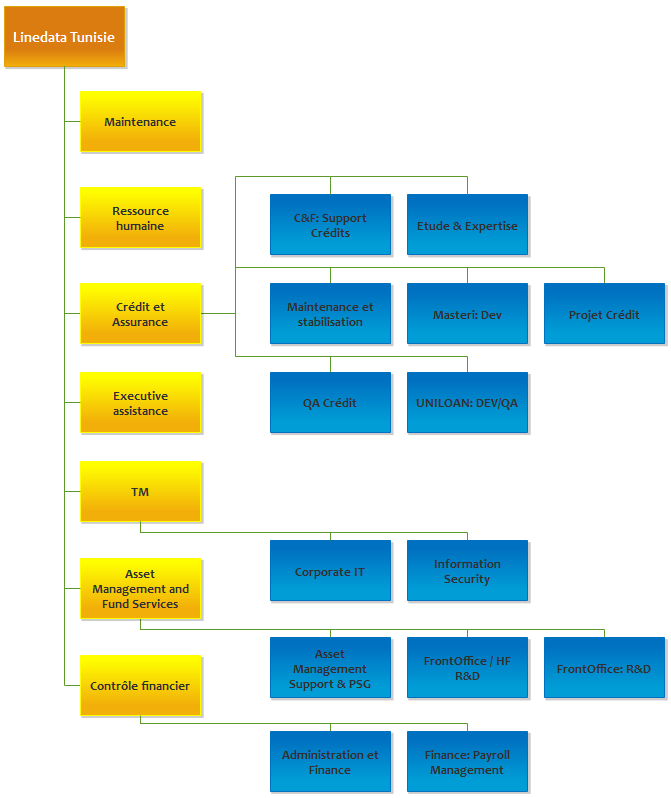
\includegraphics[scale = 1.0]{figures/Organigramme_Linedata_2.png}
  \caption{Organigramme de Linedata Tunisie}
  \label{code2}
\end{figure}


\newpage
\section{Contexte du projet}
Dans cette section, nous allons détailler les objectifs du projet ainsi que les différentes tâches à réaliser.
\subsection{Etude de l'existant}
Linedata est une société qui offre des solutions globales de qualité. De ce fait, cette dernière donne une importance majeure aux avis de ses clients. Chaque jour, elle reçoit de multiples demandes d'ajout de fonctionnalités ou des réclamations de bogue que ce soit du client ou de leurs assurances qualité. Ces réclamations sont donc triées puis distribuées aux équipes chargées de la maintenance du produit concerné. Le chef d'équipe doit alors distribuer les tâches aux membres de son équipe. Pour pouvoir les distribuer, ce dernier doit se baser sur plusieurs indicateurs de performance. Il doit en premier lieu utiliser des requêtes SQL\footnote{Structured Query Language, en français langage de requête structurée.  C'est un langage informatique normalisé servant à exploiter des bases de données relationnelles \cite{SQL}} pour extraire les données nécessaires sur chaque membre de l'équipe d'une base de données déjà existante. La figure \ref{code4} représente un exemple d'une requête SQL utilisée.
\begin{figure}[H]
  \centering
  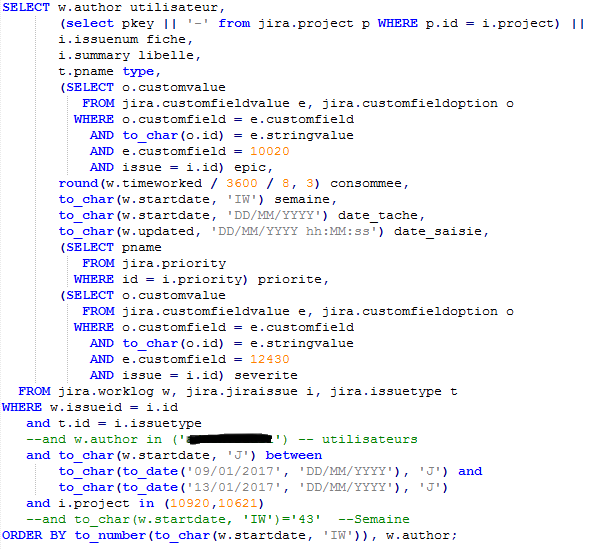
\includegraphics[scale=0.65,width=10cm]{figures/used_sql_request.png}
  \caption{Requête SQL utilisée}
  \label{code4}
\end{figure}
Puis les données sont saisies et enregistrées manuellement sous format Excel. La Figure \ref{code5} représente un exemple de feuille Excel. 
\begin{figure}[H]
  \centering
  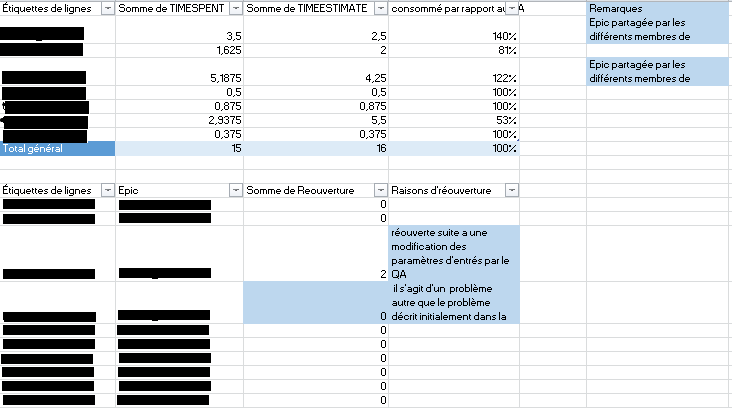
\includegraphics[scale=0.7]{figures/used_excel_file.png}
  \caption{Feuille Excel utilisée}
  \label{code5}
\end{figure}
Ensuite, le chef d'équipe calcule quelques indicateurs de performance à partir de la feuille Excel tel que le nombre de tâches traitées qui ont une certaine complexité sur le nombre de jours passés, le nombre de tâches traitées sur le nombre de jours passés regroupé par mois et le nombre de retours\footnote{Un retour sur une tâche est la non-validation de la tâche traitée et la demande de correction de cette dernière} sur le total des tâches traitées. La figure \ref{code9} représente un exemple de rapport après le calcul de l'indicateur de performance ratio des tâches par mois.
\begin{figure}[H]
  \centering
  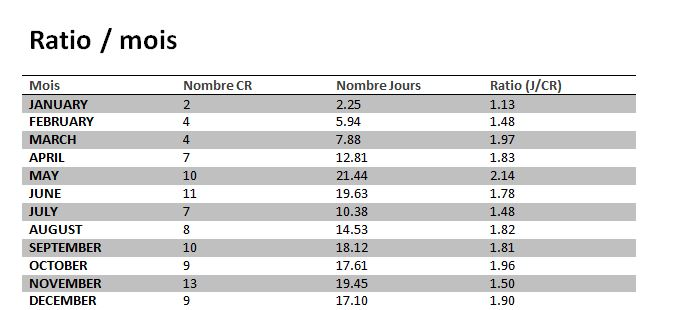
\includegraphics[scale=1.06]{figures/ratio_mois_example.jpg}
  \caption{Exemple de rapport d'indicateurs: Ratio tâches par mois}
  \label{code9}
\end{figure}
Enfin, le chef d'équipe distribue les tâches aux membres en estimant le temps nécessaire pour les finir et en s’appuyant sur les indicateurs de performance.
\subsection{Critique de l'existant}
Le responsable, ne disposant d'aucun outil d'aide pour la collecte et le calcul des indicateurs, mettait trop de temps dans la sélection des membres qui vont s'occuper d'une réclamation. En plus de cela, le risque d'erreur est toujours présent puisque le calcul se faisait de façon manuelle. Sans parler du fait que le suivi du rendement était une tâche difficile puisqu'il n'existe aucun outil de collecte d'informations sur les employés et de traitement de ces derniers dans la société.
\subsection{Présentation du projet}
Afin de faciliter la tâche du chef de projet, nous proposons une solution qui va être décomposée en deux parties: la première qui consiste à créer des tableaux de bords pour le suivi des membres de l'équipe (suivi de performances des membres avec les différents indicateurs de performance évoqués). Ces tableaux de bords vont être basés sur plusieurs indicateurs de performance tels que le nombre de jours passés dans le traitement de fiches regroupé par complexité ou le nombre de fiches traité dans une période déterminée. La seconde partie va tourner autour de l'optimisation des plannings. Et ceci en automatisant le calcul des indicateurs de performance des membres de l'équipe et en optimisant le choix des membres qui vont traiter les tâches.
Cette solution va considérablement réduire le temps que prend l'étape de sélection des membres. Elle va aussi éliminer le risque d’erreurs de calcul et de collecte de données erronées.
\section{Langage de modélisation UML}
La notation UML\footnote{Unified Modeling Language en anglais qui signifie langage de modélisation unifié} est un \textbf{langage visuel} constitué d'un ensemble de schémas, appelé des diagrammes, qui donnent chacun une vision différente du projet à traiter. UML nous permet donc de représenter le logiciel à développer sous forme de diagrammes qui définissent son fonctionnement.\cite{UMLIntroduction}\\

UML est constitué de 13 diagrammes qui représentent chacun un concept du système. Ces derniers peuvent être représentés par le schéma de 4 vues qui est axées sur les besoins des utilisateurs et qu'on appelle 4+1 vues.\\

Les besoins des utilisateurs représente le cœur de l'analyse. On y décrit le contexte, les acteurs du projet, les fonctionnalités et les interactions entre ces acteurs et ces fonctionnalités.
Les besoins peuvent être représentés à l'aide de deux diagrammes: le diagramme de packages et le diagramme de cas d'utilisation.\\

La vue logique a pour but d'identifier les éléments du domaine et les relations et interactions entre ces éléments. Cette vue organise les éléments du domaine en catégories. Deux diagrammes peuvent être utilisés: le diagramme de classes et le diagramme d'objets.\\

La vue des processus démontre la décomposition du système en processus et actions, les interactions entre les processus et la synchronisation et la communication des activités parallèles. La vue des processus peut être représentée par plusieurs diagrammes: le diagramme de séquence, le diagramme d'activité, le diagramme de collaboration, le diagramme d'état-transition, le diagramme global d'interaction et le diagramme de temps.\\

La vue des composants (vue de réalisation) permet de mettre en évidence les composant du futur système(fichiers sources, bibliothèques, base de données ou autre). Cette vue comprend deux diagrammes: le diagramme de structure composite et le diagramme de composants.\\

La vue de déploiement décrit les ressources matérielles et la répartition des parties du logiciel sur ces éléments. Cette vue contient qu'un diagramme: le diagramme de déploiement\cite{UMLDiagrams}.\\

\section{Méthodologie de travail}
Après des recherches sur les méthodes de gestion de projets nous avons choisi les méthodes agiles pour piloter le nôtre.
\subsection{Approche agile}
Le mouvement des méthodes agiles a vu le jour en 2001 aux États-Unis \cite{Agile}. Des experts dans le domaine de l'informatique se sont réunis afin de créer ces méthodes suite à un taux d'échec important des projets informatiques dans les années 1990.\\

Les méthodes agiles se reposent sur des cycles de développement itératifs et incrémentaux en fonction des besoins évolutifs du client. Ces méthodes permettent donc de mieux répondre aux attentes du client en un temps limité (grâce à l'implication de ce dernier) tout en faisant monter les collaborateurs en compétences. Ces méthodes constituent donc un gain en productivité.
Il existe plusieurs méthodes agiles telles que eXtreme Programming(XP), Crystal, Kanban ou encore Rapid Application Development (RAD). Nous avons choisi d'utiliser Scrum pour notre projet.
\subsection{Méthode Scrum}
La méthode Scrum est une méthode agile créée en 2002 dont le nom signifie littéralement "la mêlée". Elle consiste à découper le projet en des itérations qu'on nomme sprints. Un sprint a une durée qui varie entre deux à quatre semaines.
Avant chaque sprint, les tâches sont estimées en temps et en complexité et ceci pour planifier les livraisons et estimer les coûts auprès du client. Les fonctionnalités qui font objet d'un sprint (appelé user stories) constituent ce qu'on appelle sprint backlog du produit qui va être livré à la fin du sprint. Il est nécessaire de distinguer entre sprint backlog et product backlog qui est l'ensemble des fonctionnalités du produit final.\\

La méthode Scrum est caractérisée par une mêlée quotidienne, dans laquelle les membres de l'équipe indiquent les tâches qu'ils ont finies, les difficultés rencontrées et ce qu'il leur reste à faire. Cela permet d'évaluer l'avancement du projet et surtout de venir en aide à ceux qui rencontre des difficultés qu'on a déjà rencontrées auparavant.\\

La figure \ref{code3} présente une itération selon la méthode Scrum
\begin{figure}[H]
  \centering
  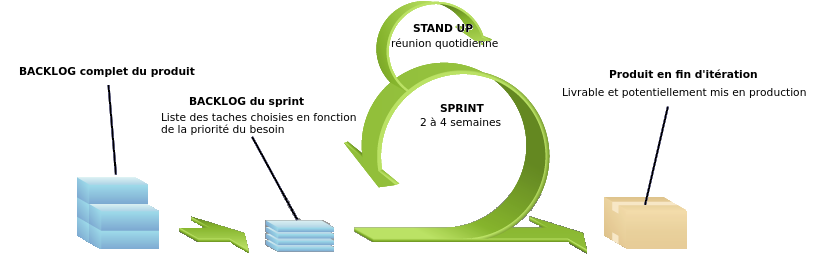
\includegraphics[scale=0.7]{figures/iteration_scrum.png}
  \caption{Itération selon la méthode Scrum}
  \label{code3}
\end{figure}

\subsubsection{Les rôles de la méthode Scrum}
La méthode Scrum définit trois rôles:\\
\begin{itemize}
\item[$\circ$] \textbf{Product Owner}: Il s'agit du représentant du client dans un projet Scrum. Il définit les besoins et les spécifications. Il est aussi chargé de définir les user stories.\\
\item[$\circ$] \textbf{Scrum master}: Il est chargé de veiller à la mise en application de la méthode et le respect de ses objectifs. C'est une personne chargée de lever les obstacles qui ralentissent l'avancement de l'équipe et du projet.\\
\item[$\circ$] \textbf{L'équipe}: Ce sont les personnes chargées de la réalisation des sprints. Il peut s'agir d'un architecte, développeur ou testeur.
\end{itemize}
\section{Conclusion}
Dans ce chapitre nous avons présenté l'organisme d'accueil. Puis, nous avons énoncé le contexte du projet. Après, nous avons défini le langage de modélisation UML et à la fin, nous avons présenté la méthode qu'on va utiliser pour la réalisation du projet. Dans le prochain chapitre, nous allons détailler les besoins de notre projet.